\documentclass[12pt,letterpaper]{article}
\usepackage{./preamble}

%%%%%%%%%%%%%%%%%%%%%%%%%%%%%%%%%%%%%%%%%%
%%%% Edit These for yourself
%%%%%%%%%%%%%%%%%%%%%%%%%%%%%%%%%%%%%%%%%%
\newcommand\course{Computational Statistics}
\newcommand\hwnumber{2}
\newcommand\userID{Davi Sales Barreira}
\DeclareRobustCommand{\rchi}{{\mathpalette\irchi\relax}}
\newcommand{\irchi}[2]{\raisebox{\depth}{$#1\chi$}}
\newcommand*{\QEDA}{\hfill\ensuremath{\blacksquare}}%

\begin{document}
% \textbf{\Large Worksheet completed with Octave.}

\section*{Exercise 1 (Monte Carlo for Gaussians)}
\begin{enumerate}[leftmargin=!,labelindent=5pt]
	\item Let's prove that $E[\phi(X)] = E[\phi(X+\theta)
	exp(\frac{-1}{2}\theta^T\theta - \theta^T X)]$.
	% $$ E[\phi(X)] = \int_{\mathbb{R}^d} \phi(x) \pi(x) dx_1...dx_d$$

	$$ E[\phi(X+\theta)exp(\frac{-1}{2}\theta^T\theta - \theta^T X)]
	= \int_{\mathbb{R}^d} \phi(x+\theta) exp(\frac{-1}{2}\theta^T
	\theta - \theta^T x)\pi(x)dx_1...dx_d = $$

	$$ =  \int_{\mathbb{R}^d} \phi(x+\theta) exp\left(\frac{-1}{2}
	\theta^T
	\theta - \theta^T x \right)exp(-x^T x / 2)\frac{1}{(\sqrt{2\pi})^d}
	dx_1...dx_d = $$

	$$ \int_{\mathbb{R}^d} \phi(x+\theta) exp\left(\frac{-1}{2}
	(x-\theta)^T(x-\theta)\right)\frac{1}{(\sqrt{2\pi})^d}
	dx_1...dx_d$$

	Finally, making $x-\theta = y$,
	$$ \int_{\mathbb{R}^d} \phi(y) exp\left(\frac{-1}{2}
	(y)^T(y)\right)\frac{1}{(\sqrt{2\pi})^d}
	dy_1...dy_d = E[\phi(Y)] $$
	\qed


	\item Let's show that
	$$ \sigma^2(\theta) = E\left[ 
	\phi^2(X) exp\left(
		\frac{-1}{2}X^T X + \frac{1}{2}(X - \theta)^T(X - \theta)
		\right)
	\right] - E[\phi(X)]^2$$

	Note that, using the result in the previous item we have:
	$$ \sigma^2(\theta) = V\left[
	\phi(X + \theta)exp\left(
		\frac{-1}{2}\theta^T \theta - \theta^T X
		\right)
	\right] = $$

	$$
	= E \left[ \left(
	\phi(X + \theta)exp\left(
		\frac{-1}{2}\theta^T \theta - \theta^T X
		\right) \right ) ^ 2
	\right] -
	E \left[
	\phi(X + \theta)exp\left(
		\frac{-1}{2}\theta^T \theta - \theta^T X
		\right)
	\right] ^2  = 
	$$

	$$
	= E \left[ \left(
	\phi(X + \theta)exp\left(
		\frac{-1}{2}\theta^T \theta - \theta^T X
		\right) \right ) ^ 2
	\right] -
	E \left[ \phi(X)
	\right] ^2
	$$
	Now, let's rearrange the first term in the variance.
	$$ \sigma^2(\theta) = 
	\int_{\mathbb{R}^d} \phi(x+\theta)^2 exp\left(
	 - \theta^T
	\theta - 2\theta^T X \right)exp(-x^T x / 2)\frac{1}{(\sqrt{2\pi})^d}
	dx_1...dx_d = $$

	Make $X + \theta = Y$, then:

	$$
	\int_{\mathbb{R}^d} \phi(y)^2 exp\left(
	 - \theta^T
	\theta - 2\theta^T (y-\theta) \right)exp(-(y-\theta)^T (y-\theta) / 2)
	\frac{1}{(\sqrt{2\pi})^d}
	dy_1...dy_d = $$

	$$ = 
	\int_{\mathbb{R}^d} \phi(y)^2 exp\left(
	\frac{1}{2}(y-\theta)^T(y-\theta) - \frac{y^Ty}{2}
	\right)
	exp \left( \frac{-y^Ty}{2}
	\right)
	\frac{1}{(\sqrt{2\pi})^d}
	dy_1...dy_d = $$
	$$ 
	= E\left[ 
	\phi^2(X) exp\left(
		\frac{-1}{2}X^T X + \frac{1}{2}(X - \theta)^T(X - \theta)
		\right)
	\right]
	$$

	Therefore, 
	$$ \sigma^2(\theta) = E\left[ 
	\phi^2(X) exp\left(
		\frac{-1}{2}X^T X + \frac{1}{2}(X - \theta)^T(X - \theta)
		\right)
	\right] - (E[\phi(X)]^2 $$ \qed



	\item Let's calculate $\nabla ^2\sigma^2(\theta) = H(\theta)$.
	$$
	\frac{\partial \sigma^2(\theta)}{\partial \theta_i} =
	\frac{\partial E[\phi(X)^2exp(\frac{-X^T X+(X-\theta)^T(X-\theta)}{2} )]}
	{\partial \theta_i} =
	$$
	$$
	= \int_\chi \phi(x)^2 exp(-x^Tx)
	\frac{\partial}{\partial \theta_i}
	exp \left(\frac{(x-\theta)^T(x-\theta)}{2}\right)
	\frac{1}{(\sqrt{2\pi})^d}
	dx = 
	$$
	$$
	= \int_\chi \phi(x)^2 exp(-x^Tx)
	(\theta_i - x_i)
	exp \left(\frac{(x-\theta)^T(x-\theta)}{2}\right)
	\frac{1}{(\sqrt{2\pi})^d}
	dx
	$$

	We calculated the gradient, let's now calculate the second derivative.
	First the diagonal.
	$$
	\frac{\partial}{\partial \theta_i}\int_\chi \phi(x)^2 exp(-x^Tx)
	(\theta_i - x_i)
	exp \left(\frac{(x-\theta)^T(x-\theta)}{2}\right)
	\frac{1}{(\sqrt{2\pi})^d}
	dx =
	$$
	$$
	 = E[\phi(X)^2] + \int_\chi \phi(x)^2 exp(-x^T x)
	exp\left(\frac{(x - \theta)^T(x - \theta)}{2}\right)
	(x_i-\theta_i)(x_i - \theta_i)
	\frac{1}{(\sqrt{2\pi})^d}dx
	$$

	Now the rest:
	$$
	\frac{\partial}{\partial \theta_j}\int_\chi \phi(x)^2 exp(-x^Tx)
	(\theta_i - x_i)
	exp \left(\frac{(x-\theta)^T(x-\theta)}{2}\right)
	\frac{1}{(\sqrt{2\pi})^d}
	dx =
	$$
	$$
	 = \int_\chi \phi(x)^2 exp(-x^T x)
	exp\left(\frac{(x - \theta)^T(x - \theta)}{2}\right)
	(x_i-\theta_i)(x_j - \theta_j)
	\frac{1}{(\sqrt{2\pi})^d}dx
	$$
	\qed

	\item We already know that the Hessian is positive definite. Hence,
	we only need to show that the derivative is equal to zero at
	$\theta^*$.

	$$\nabla \sigma^2(\theta) =
	\int_\chi \phi(x)^2 exp(-x^Tx)(\theta - x)
	exp \left(\frac{-(x-\theta)^T(x-\theta)}{2} \right)
	\frac{1}{(\sqrt{2\pi})^d}dx = 
	$$
	$$
	= 	
	\int_\chi \phi(x)^2 exp(-x^Tx)(\theta - x)
	exp \left(\frac{-(x-\theta)^T(x-\theta)}{2} \right)
	\frac{1}{(\sqrt{2\pi})^d}dx = 
	$$
	$$
	= 
	\int_\chi \phi(x)^2 (\theta - x)
	exp \left(\frac{-x^Tx}{2} - \theta^Tx
	+ \frac{-\theta^T\theta}{2}\right)
	\frac{1}{(\sqrt{2\pi})^d}dx = 
	$$
	$$
	= 
	\int_\chi \phi(x)^2 (\theta - x)
	exp(-\theta^Tx)exp(-x^Tx/2)
	\frac{exp(\theta^T\theta/2)}{(\sqrt{2\pi})^d}dx =  0
	$$
	Finally, since the last term doens't depend on $X$, we can eliminate
	it, obtaining:

	$$ E[\phi(X)^2(\theta^* -X)exp(-\theta^{*T}X)] = 0$$
	\qed

	\item Couldn't solve.
\end{enumerate}

\newpage
\section*{Exercise 2 (Metropolis-Hastings)}
\begin{enumerate}[leftmargin=!,labelindent=5pt]
\item First, generate $Y \sim q(X_t, \cdot)$. 
With probability equal to $\alpha(x,y)$, make $X_{t+1} = Y$, and with
probability $1 - \sum_{z \in \mathbb Z} \alpha(x,z)q(x,z)$ make
$X_{t+1} = X_t$. Then, repeat the process.

\item We want to show that $\pi(x)T(x,y) = \pi(y)T(y,x)$.
For $y=x$, this is trivial. Now, assume $y\neq x$. Therefore:
$$
\pi(x)T(x,y) = \pi(x)\alpha(x,y)q(x,y) =
\pi(x)\frac{\gamma(x,y)}{\pi(x)q(x,y)}q(x,y) = \gamma(y,x) =
$$
$$
= 
\pi(y)\frac{\gamma(y,x)q(y,x)}{\pi(y)q(y,x)} = \pi(y)T(y,x)
$$
\qed


\item Using Metropolis-Hastings, one has:
$$ \alpha = min \left\{ 
1, \frac{\pi(x^*)q(x_{t-1} \mid x^*)}{\pi(x_{t-1})q(x^*\mid x_{t-1})}
\right\}$$
% So, $\alpha(x,y) = \frac{\gamma(x,y)}{\pi(x)q(x,y)}$, for
Note that 
$x = x_{t-1}, x^* = y, q(x,y) = q(x^* \mid x_{t-1})$.

Now make:
$$ \gamma(x,y) = max \left\{ 
\pi(y)q(y,x),\pi(x)q(x,y)
\right\}$$
$$ \therefore $$
$$\alpha(x,y) =
\frac{max\{ \pi(y)q(y,x), \pi(x)q(x,y)\}}{\pi(x)q(x,y)} = 
$$
$$ = min \left\{ 
1, \frac{\pi(y)q(y,x)}{\pi(x)q(x,y)}
\right\}$$
\qed

\item First, let's rewrite the estimate as a function of $Y$.
Note that $Y^{(k)} = X^{(\tau_k)}$ and our estimate is:
$$
\frac{1}{\tau_k - 1} \sum_{t=1}^{\tau_k-1} \phi(X^{(t)})
$$
$Y$ is the sequence of values accepted in the M-H algorithm, while
$X$ is the sequence containing all values, even when the chain
didn't move. For example:
$$
(X_t) = [0,1,1,1,2,3,3,1]
$$
$$
(Y_t) = [0,1,2,3,1]
$$

$$
\tau_1 = 1 \implies Y^{(1)} = X^{(1)} = 0
$$
$$
\tau_3 = 5 \implies Y^{(3)} = X^{(5)} = 2
$$
Hence, our estimator is the average of
$\phi(X)$ until the time $\tau_k - 1$. To write it in terms of $Y$,
each value of $Y^{(k)}$ must be multiplied by the number of times
the chain stayed in that value. Therefore:
$$
\frac{1}{\tau_k - 1} \sum_{t=1}^{\tau_k-1} \phi(X^{(t)}) =
\frac{1}{\tau_k - 1} \sum_{t=1}^{k-1} \phi(Y^{(t)})
(\tau_{t+1} - \tau_{t})
$$


Now, let's prove it has the desired transition kernel.
$$
K(x,y) = P(Y^{(k)}= y \mid Y^{(k-1)}=x) =
P(X^{(\tau_k)}=y \mid X^{(\tau_k -1)}=x)
$$

The event $X^{(\tau_k)}=y \mid X^{(\tau_k -1)}=x$ is equivalent
to moving from $x$ to $y$ and then accepting $y$, hence
$q(x,y)\cdot \alpha(x,y) \propto P(X^{(\tau_k)}=y \mid X^{(\tau_k -1)}=x)$.

Therefore, we just normalize to get the proper equation
$$P(Y^{(k)}= y \mid Y^{(k-1)}=x) =
\frac{q(x,y)\alpha(x,y)}{\sum_{z \in \mathbb Z}\alpha(x,z)q(x,y)}$$
\qed

\item Let's show that
$
\tilde{\pi}(x)K(x,y) = \tilde{\pi}(y)K(y,x)
$.

$$
\frac{\pi(x)m(x)}{\sum_{z \in \mathbb{Z}}\pi(z)m(z)} \cdot 
\frac{q(x,y)\alpha(x,y)}{\sum_{z \in \mathbb{Z}}\alpha(x,z)q(x,z)}
=
\frac{\pi(x)q(x,y)\alpha(x,y)}
{\sum_{z \in \mathbb{Z}}\pi(z)m(z)}
$$
Note that $\alpha(x,y) =
\frac{\gamma(x,y)}{\pi(x)q(x,y)} =
\frac{\gamma(y,x)}{\pi(x)q(x,y)}$. Therefore:
$$
\frac{\pi(x)q(x,y)\gamma(x,y)}
{\alpha(x,z)q(x,z)\sum_{z \in \mathbb{Z}}\pi(z)m(z)} = 
\frac{\gamma(y,x)}
{\sum_{z \in \mathbb{Z}}\pi(z)m(z)} =
\frac{\alpha(y,x)\pi(y)q(y,x)}{\sum_{z \in \mathbb{Z}}\pi(z)m(z)}=
\tilde{\pi}(y)K(y,x)
$$
\qed

\item Couldn't solve.

\end{enumerate}

\newpage
\section*{Exercise 3 (Metropolis-Hastings)}
\begin{enumerate}[leftmargin=!,labelindent=5pt]

\item Let's show that
$\int_\chi \pi(x)(\alpha(x)q(y) (1-\alpha(x)))\delta_x(y) dx = \pi(y)$.
Note that, $\pi(x) = \frac{q(x)}{\alpha(x)Z_\pi}$, hence:

$$
\int_\chi \pi(x)(\alpha(x)q(y) (1-\alpha(x)))\delta_x(y) dx =
\int_\chi \frac{q(x)}{\alpha(x)Z_\pi}(\alpha(x)q(y) (1-\alpha(x)))
\delta_x(y) dx = 
$$
$$ = 
\int_\chi \frac{q(x)}{\alpha(x)Z_\pi}\alpha(x)q(y) dx +
\pi(y)(1-\alpha(y)) = 
\frac{q(y)}{Z_\pi}\int_\chi q(x)dx +\pi(y)(1-\alpha(y)) =
$$
$$
 = \pi(y)\alpha(y) + \pi(y)(1-\alpha(y)) = \pi(y)
$$
\qed

\item Note that $X_t = \alpha X^* + (1-\alpha)X_{t-1}$, where
$X^* \sim q(\cdot)$ and $\alpha$ is the probability of acceptance
. Hence:
$$
Cov(X_1,X_2) = Cov(X_1,\alpha X^* + (1-\alpha)X_{1})=
Cov(X_1,\alpha X^*) + (1-\alpha)Cov(X_1,X_1)
$$
Since the value of $X^*$ is not correlated with the previous step,
we get:
$$Cov(X_1,X_2) = (1-\alpha) \mathbb V(X_1)$$
Using recursion, we have:
$$Cov(X_1,X_k) = (1-\alpha)^{k-1} \mathbb V(X_1)$$
$$
\sigma_X^2 = \mathbb V(X_1) + 2\sum_{k=2}^\infty Cov(X_1,X_k)=
\mathbb V(x_1) + 2\mathbb V(X_1)
\sum_{k=2}^\infty (1-\alpha)^{k-1}=
$$

$$
=
\mathbb V(x_1) + 2\mathbb V(X_1)
\sum_{m=1}^\infty (1-\alpha)^{m}=
\mathbb V(x_1) + \frac{2\mathbb V(X_1)}{\alpha}
$$
\qed


\end{enumerate}

\newpage
\section*{Exercise 4 (Gibbs Sampler)}
\begin{enumerate}[leftmargin=!,labelindent=5pt]
\item 
$$
\pi(x \mid y) = \frac{\pi(x,y)}{\pi(y)} \propto
\frac{exp((x-1)^2(y-2)^2)/2}{(y-2)^{-1}} \sim N(1,(y-2)^{-2})
$$
Now, follow the same procedure to for $\pi(y \mid x)$, hence:
$$
\pi(y\mid x) \sim N(2, (x-1)^{-2})
$$
\qed

\item The sampler doesn't make sense, because:
$$
\int_{-\infty}^{\infty}
\int_{-\infty}^{\infty}
\pi(x,y)dxdy \propto
\int_{-\infty}^{\infty}
\int_{-\infty}^{\infty}
exp((x-1)^2(y-2)^2)/2 dx dy =
$$
$$ = 
\int_{-\infty}^{\infty}
\sqrt{2\pi}((y-2)^{-2})^{\frac{1}{2}}dy = \infty
$$
\qed

\end{enumerate}

\newpage
\section*{Exercise 5 (Gibbs Sampler)}
\begin{enumerate}[leftmargin=!,labelindent=5pt]
\item  
$$
p(Z_i = z \mid \theta_1, \theta_2) = p(X_i + Y_i = z \mid
\theta_1,\theta_2) =
\sum_{y = 0}^{z}p(X_i+Y_i = z \mid Y_i = y, \theta_1,\theta_2)
p(Y_i = y \mid \theta_2) =
$$
$$ = 
\sum_{y = 0}^{z}p(X_i = z - y \mid \theta_1 )p(Y_i = y\mid\theta_2) =
\sum_{y = 0}^{z}\binom{m_i}{z-y}
\theta_1^{z - y}(1-\theta_1)^{m_i - (z-y)}
\binom{n_i}{y}
\theta_2^{y}(1-\theta_2)^{n_i - y} \therefore
$$
$$
p(Z_1,...,Z_T \mid \theta_1, \theta_2) = 
\prod_{i=1}^{T}\left ( 
\sum_{y_i = 0}^{z_i}\binom{m_i}{z_i-y_i}
\theta_1^{z_i - y_i}(1-\theta_1)^{m_i - (z_i-y_i)}
\binom{n_i}{y_i}
\theta_2^{y_i}(1-\theta_2)^{n_i - y_i}
\right)
$$
\qed

\item To sample from
$
p(\theta_1,\theta_2 \mid Z_1,...,Z_T)
$
we will use auxiliary varibles $X_{1:T}, Y_{1:T}$. 
$$
p(\theta_1 \mid \theta_2, X_{1:T},Y_{1:T},Z_{1:T}) \propto 
\pi(\theta_1 \mid \theta_2, Y_{1:T})
p(X_{1:T} \mid \theta_1,\theta_2, Y_{1:T}) \propto
$$
$$
\propto 
\pi(\theta_1)p(X_{1:T}\mid \theta_1) \propto
\theta_1^{\sum x_i}(1-\theta_1)^{\sum m_i - x_i} \therefore
$$

$$
\theta_1 \mid X_{1:T} \sim Beta \left(
1 + \sum_{i=1}^T x_i, 1 + \sum_{i=1}^T m_i - x_i
\right)
$$

Similarly to $\theta_2$:
$$
\theta_2 \mid Y_{1:T} \sim Beta \left(
1 + \sum_{i=1}^T y_i, 1 + \sum_{i=1}^T n_i - y_i
\right)
$$
Finally,
$$
p(X_{1:T},Y_{1:T} \mid \theta_1, \theta_2, Z_{1:T}) \propto
\prod_{i=1}^{T}\binom{m_i}{x_i}\theta_1^{x_i}(1-\theta_1)^{m_i - x_i}
\binom{n_i}{y_i}\theta_2^{y_i}(1-\theta_2)^{n_i - y_i}
\mathbb{I}_{\{
x_i + y_i = z_i
\}}
$$
Note that we can now use a Gibbs sampler by first
sampling $\theta_1^{(0)}$
and  $\theta_2^{(0)}$ from independent $U_{[0,1]}$. Secondly, we can sample
$X^{(0)}$ and $Y^{(0)}$ from $p(X_{1:T},Y_{1:T}
\mid \theta_1^{(0)}, \theta_2^{(0)}, Z_{1:T})$,
since the distribution found is discrete with finite 
support, hence, we can calculate the probabilty for each possible value
of $X^{(0)}$ and $Y^{(0)}$.
With the values for the auxiliary variables, we 
sample $\theta_1^{(1)}$ and $\theta_2^{(1)}$ from their posteriors, which is possible
since they are Beta distributions. Again we sample $X,Y$ using the
updated $\theta_1,\theta_2$ and repeat the process.
\qed

\end{enumerate}

\newpage
\section*{Simulation question (Normal mixture model - Gibbs sampling)}
\begin{enumerate}[leftmargin=!,labelindent=5pt]
\item  
$$
P(X_i = x_i \mid p,\mu, \sigma^2) =
\sum_{z_i = 1}^{k}P(X_i = x_i \mid Z_i = z_i, p, \mu, \sigma^2)
P(Z_i = z_i \mid p,\mu, \sigma^2) = 
$$
$$ = 
\sum_{z_i = 1}^{k}\varphi(x_i; \mu_{z_i}, \sigma^2_{z_i})p_{z_i}
$$
\qed

\item 

$$
P(Z_i = z_i \mid X_i, p, \mu, \sigma^2) \propto
P(X_i \mid Z_i, p, \mu, \sigma^2)P(Z_i \mid, p, \mu, \sigma^2)
\propto
$$
$$
\varphi(x_i; \mu_{z_i},\sigma^2_{z_i}) p_{z_i} \propto
\frac{exp \left(
\frac{-(x_i-\mu_{z_i})^2}{2\sigma^2_{z_i}}
\right)}{\sqrt{2\pi\sigma^2_{z_i}}} p_{z_i}
$$

The above distribution is discrete with finite support, hence,
one can calculate the value for each $z_i$ and then normalize
by the sum, obtaining a probability mass function from which
values can be sampled.
\qed

\item
$$
P(p \mid X, Z, \mu, \sigma^2) \propto
P(X,Z \mid \mu, \sigma^2, p) P(p \mid \mu, \sigma^2) \propto
P(X \mid Z, \mu, \sigma^2, p)P(Z \mid \mu, \sigma^2, p)\pi(p)
$$
Note that
$P(X \mid Z, \mu, \sigma^2, p) \propto
\prod_{i=1}^N\phi(x_i;\mu_i,\sigma^2_i)$ is not a function
$p$, so it can be thrown as a constant. Also, 
$P(Z \mid \mu, \sigma^2, p) = P(Z \mid p)$
therefore:
$$
P(p \mid X, Z, \mu, \sigma^2) \propto
\pi(p) \prod_{i=1}^N p_{z_i} \propto
\prod_{j=1}^K p_j^{\gamma_j -1}\prod_{i=1}^N p_{z_i} 
$$

Let $n_j = \sum_{i=1}^N z_i \mathbb I_{z_i = j}$, so $n_j$ is
the number of times the $j$-th Gaussian has being picked. Finally:

$$
P(p \mid X, Z, \mu, \sigma^2) \propto
\prod_{j=1}^K p_j^{\gamma_j -1 + n_j} 
$$
$$
p \mid X, Z, \mu, \sigma^2 \sim Dirichlet
$$

Since the distribution is a Dirichlet, it is known how to
sample from it.
\qed

\item
$$
P(\mu \mid X, Z, p, \sigma^2) \propto
P(X,Z \mid \mu, p, \sigma^2)P(\mu \mid p, \sigma^2) \propto
$$
$$
P(X \mid Z, \mu, p, \sigma^2)P(Z \mid \mu, p, \sigma^2)\pi(\mu) \propto
$$
$$
\left(
\prod_{j=1}^N exp \left(
	\frac{-(x_j - \mu_{z_j})^2 p_{z_j}}{2\sigma^2_{z_j}}
	\right)
\right)
\prod_{k=1}^K exp \left(
	\frac{-(\mu_k - m)^2}{2\tau^2}
\right) \propto
$$
$$
\prod_{k=1}^K
p_k^{n_k}
exp \left(
	\frac{-\sum_{i=1}^{n_k}(x_i^{(k)} - \mu_k)^2}{2\sigma_j^2} -
	\frac{(\mu_k - m)^2}{2\tau^2}
\right)
$$
$$\therefore$$

$$
P(\mu_k \mid X, Z, p, \sigma^2) \propto
exp \left(
	\frac{-\sum_{i=1}^{n_k}(x_i^{(k)} - \mu_k)^2}{2\sigma_k^2} -
	\frac{(\mu_k - m)^2}{2\tau^2}
\right)
$$
First, note that $x_i^{(k)}$ is the $i$-th value from $X$ such
that $z = k$, in other words, it is the $i$-th sampled value that came
from the $k$-th Gaussian distribution.

Note that the above equation is the same as updating each
Normal
prior distribution $\mu_k \sim N(m, \tau^2)$ and
$X^{(k)} \mid \mu_k \sim N(\mu_k, \sigma^2_k)$ with $\sigma^2_k$ known.
Therefore, let $\bar{x_k}$ be the sample average, then:
$$\mu_j \mid X, Z, p,\sigma^2
\sim N\left(
\frac{n_k \sigma_k ^{-2}\bar{x_k} + \tau^{-2}m}
{\tau^{-2} + n_k\sigma^{-2}_k}
, [n_k\sigma_k^{-2} + \tau^{-2}]^{-1}
\right)$$
\qed

\item 

$$
P(\sigma_k ^2 \mid X, Z, p, \mu) \propto
P(X \mid Z, p, \mu, \sigma_k^2) P(Z \mid p) \pi(\sigma_k^2)
\propto
$$

$$
\frac{p_k^{n_k} exp\left(
	\frac{-\sum_{i=1}^{n_k}(x_i - \mu_k)^2}{2\sigma^2_k}
\right)}
{\sigma_k^{n_k}}
\sigma_k^{-\alpha -1}exp(-\beta \sigma_k^{-2}) \propto
$$
$$
exp \left( 
\left [
	\frac{-\sum_{i=1}^{n_k}(x_i - \mu_k)^2}{2}
	- \beta
\right] \sigma_k^{-2}
\right)
\sigma_k^{-\alpha -1 - \frac{n_k}{2}} \sim
\text{Inverse Gamma}\left(
\alpha + \frac{n_k}{2}, \beta +
\frac{\sum_{i=1}^{n_k}(x_i - \mu_k)^2}{2}
\right)
$$

To sample from the Inverse Gamma, just sample $Y$ from a Gamma with these
parameters and then do $Y^{-1}$.

\item To sample $(y_1,...,y_N)$ from a mixture model,
use $p = (p_1,...,p_k)$ to sample $Z = (z_1,...,z_k)$. Then,
sample each $y_i$ from $N(\mu_{z_i},\sigma^2_{z_i})$.
\begin{figure}[H]
    \centering
    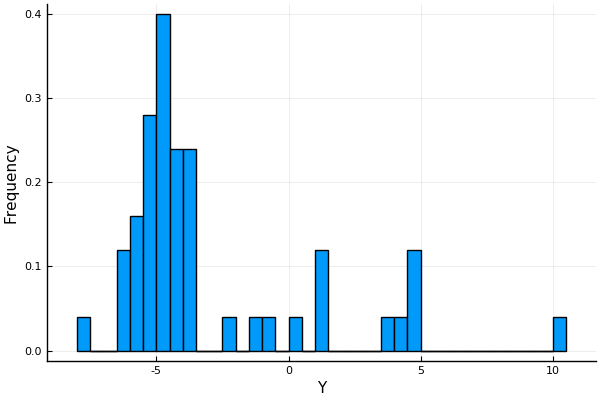
\includegraphics[width=10cm]{images/Ex6.png}
    \caption{Histogram for 500 samples from
    Gaussian Mixture model with
    $\mu = (-2, 2),\sigma^2 =(1,1), p = (0.7,0.3)$.
    }
    \label{fig:1}
\end{figure}

\item The ideia of empirical bayes
is to use the maximum-likelihood estimates
to set the parameters of the priors. We will only use the
sample average to set $m$, the location parameter for the
prior distribution of $\mu$. For the other hyperparameters,
we will chose them as to make the priors non-informative. Therefore:
$$\mu_k \sim N(m = -0.86,\tau = 100)$$
$$\sigma^2_k \sim IG(\alpha = 0.01,\beta = 0.01)$$
$$p \sim Dirichlet(\gamma_1 =1,\gamma_2 = 1)$$

\item The following steps were used in the implementation of the Gibbs
sampler:

\begin{itemize}
	\item Sample the initial values from the priors;	
	\subitem Sample $p^{(0)}$ from a Dirichlet with parameters $\gamma$;
	\subitem Sample each $\mu_k^{(0)} \sim N(m, \tau)$ and each
$(\sigma_k^2)^{(0)} \sim IG(\alpha, \beta)$;

\item Enter loop and start sampling from the full conditionals;
	\subitem Sample each $Z_i^{(t)} \mid
	p^{(t-1)},X_i,\mu^{(t-1)},(\sigma^2)^{(t-1)}$;
	\subitem Sample $p^{(t)} \mid Z^{(t)}$
	\subitem Sample $\mu^{(t)} \mid Z^{(t)},(\sigma^2)^{(t-1)},X$
	\subitem Sample $(\sigma^2)^{(t)}
	\mid Z^{(t)},(\mu)^{(t)},X$
\end{itemize}

Below we show the results of the simulation:

\begin{figure}[H]
    \centering
    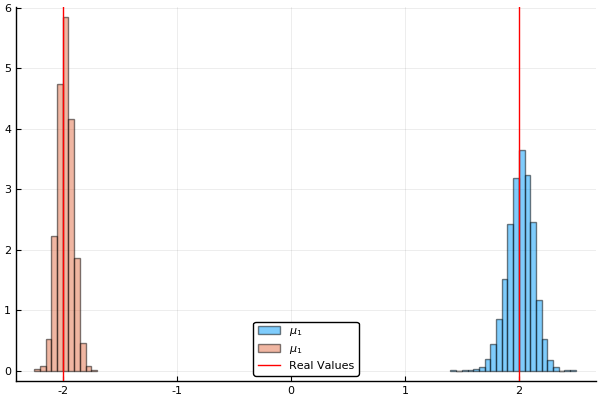
\includegraphics[width=10cm]{images/Ex8_1.png}
    \caption{Posterior distribution of $\mu$.
    }
    \label{fig:2}
\end{figure}

\begin{figure}[H]
    \centering
    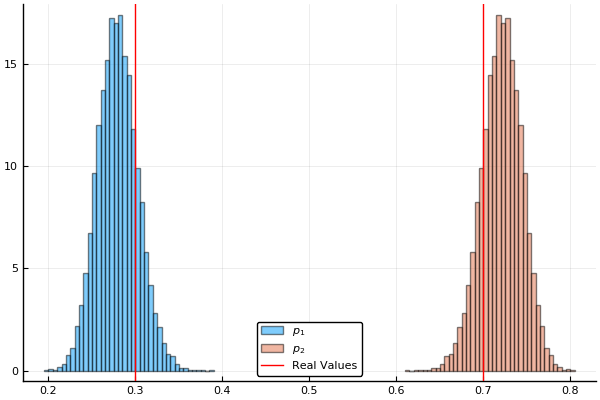
\includegraphics[width=10cm]{images/Ex8_2.png}
    \caption{Posterior distribution of $p$.
    }
    \label{fig:3}
\end{figure}
\begin{figure}[H]
    \centering
    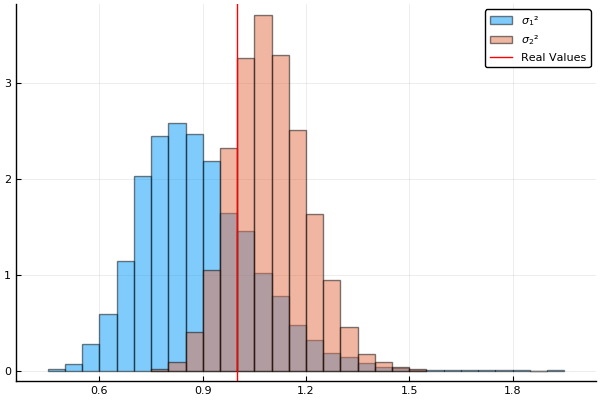
\includegraphics[width=10cm]{images/Ex8_3.png}
    \caption{Posterior distribution of $\sigma^2$.
    }
    \label{fig:4}
\end{figure}
\begin{figure}[H]
    \centering
    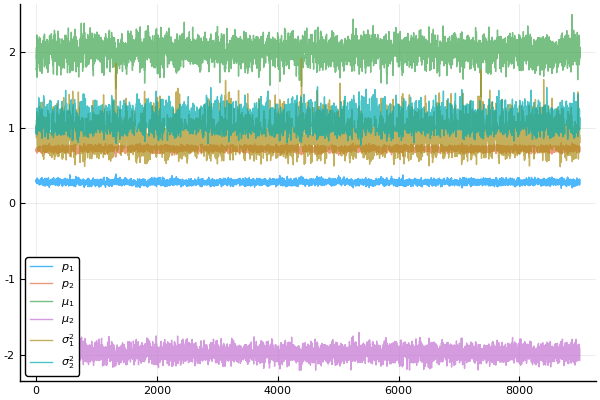
\includegraphics[width=10cm]{images/Ex8_4.png}
    \caption{Trace plot of the sampler for each parameter
    }
    \label{fig:4}
\end{figure}

\end{enumerate}

\end{document}
